\documentclass[11pt]{article}
\usepackage[margin=1in]{geometry}
\usepackage{amsmath,amssymb,amsthm}
\usepackage{hyperref}
\usepackage{booktabs}
\usepackage{graphicx}
\usepackage{microtype}
\usepackage[numbers,sort&compress]{natbib}
\usepackage{tikz}
\usetikzlibrary{arrows.meta,positioning,fit,shapes.geometric}

\hypersetup{
  colorlinks=true,
  linkcolor=blue!70!black,
  citecolor=blue!70!black,
  urlcolor=blue!70!black
}

\newtheorem{proposition}{Proposition}
\newtheorem{assumption}{Assumption}
\newtheorem{remark}{Remark}
\newtheorem{observation}{Observation}

\title{Closing the Handshake Gap: Toward a Scale-Invariant\\
Port-Hamiltonian Safety Architecture, with\\
Extreme-Case Instantiation in Medical Microrobotics}

\author{Durga Deepak Valluri\thanks{\texttt{durgadeepak.valluri97@gmail.com}}
\and
Durga Prasad Sarilla\thanks{\texttt{dpsarilla@ksu.edu}, Kansas State University}}

\date{}

\begin{document}
\maketitle

\begin{abstract}
This paper proposes the Energetics-Aware Hamiltonian Control (EA-HC) framework, a
vertically integrated architecture designed to resolve the ``Handshake Gap'': the structural
decoupling between high-level symbolic intent and low-level physical safety. While the
individual components of energy-aware robotics are well-supported in existing literature,
a unified stack bridging task-level semantics and physical thermodynamics remains an
unaddressed gap. The proposed four-layer architecture translates symbolic task requirements
into thermodynamic energy budgets, managed by a safe reinforcement learning layer and
enforced through port-Hamiltonian (pH) energy tanks.

The primary aim is to investigate the plausibility of a scale-invariant control architecture
in which deterministic passivity acts as a universal safety veto across diverse robotic embodiments. Medical microrobotics in stochastic, Brownian-dominated environments is selected
as an extreme-case instantiation to examine whether the architecture remains well-defined
and evaluable at the boundary of its operating range. The physical plant is modeled as a
Stochastic Port-Hamiltonian System (SPHS), and the admissibility condition is extended by
two stochastic energy buffers: an It\^{o} correction and a L\'{e}vy jump correction, both derived
directly from the It\^{o}--L\'{e}vy formula. The scope of the thermodynamic veto is explicitly
bounded: it enforces passivity against the robot's own actuator outputs and internally
generated stochastic disturbances. Geometric confinement against exogenous ambient forces
(e.g., pulsatile blood-flow drift) is a distinct safety objective treated as future work.

This work proposes a foundation for further investigation into the EA-HC architecture as
a scale-invariant framework unifying symbolic reasoning and physical safety across the full
spectrum of robotic embodiments.

\smallskip
\noindent\textbf{Note:} Numerical simulation and hardware experiments are ongoing and will be reported in a subsequent version.
\end{abstract}

\tableofcontents
\newpage

\section{Introduction}

Modern robotics confronts a fundamental architectural tension. High-level task planners and
reinforcement learning (RL) policies reason in the currency of symbolic rewards, abstract
goals, and discrete state transitions \cite{kober2013,levine2016}. Physical actuators, by contrast, obey the laws of
thermodynamics: energy must be conserved, dissipated, or stored, and passivity violations
manifest as unstable oscillations, mechanical failure, or harm to human operators and biological
tissue \cite{vanderschaft2014,ferraguti2013}.

We term this decoupling the \emph{Handshake Gap}: the absence of a shared language that allows a
high-level intent to be continuously translated into a physically valid actuation budget. The
gap is not merely an implementation inconvenience; it is a structural safety hazard. A policy
that hallucinates an optimal trajectory that is energetically infeasible will, in the absence of a
physical veto, attempt to execute that trajectory through the actuators.

Existing approaches address fragments of this problem. Energy-aware control \cite{ferraguti2015,schindlbeck2015} enforces
passivity locally but does not connect to semantic task layers. Safe RL via Constrained Markov
Decision Processes (CMDPs) \cite{garcia2015,altman1999} learns safety boundaries statistically but cannot guarantee
thermodynamic admissibility in closed form. Port-Hamiltonian systems \cite{vanderschaft1995,maschke1992} provide a principled
energy substrate but are not typically integrated with learning-based intent layers.

\paragraph{Scope clause.} The EA-HC framework addresses the Handshake Gap by establishing energy as
the universal safety currency between the symbolic and physical layers. The thermodynamic veto
enforces passivity against the robot's own actuator actions and internally generated stochastic
disturbances. It does not, in its current form, guarantee spatial confinement against exogenous
ambient forces (e.g., pulsatile blood flow, pressure gradients, or vessel-wall collisions). Geometric
safety against such forces is a distinct objective and is identified as the primary direction for
future work (Section~\ref{sec:conclusion}).

\paragraph{Contributions.} This paper makes the following contributions:
\begin{enumerate}
\item \textbf{Jump-diffusion SPHS extension.} We extend the stochastic port-Hamiltonian
  formulation of Cordoni et al.\ \cite{cordoni2022} -- which covers general continuous
  semimartingales (excluding jump-discontinuous noise) -- to the jump-diffusion regime by
  incorporating a compensated Poisson random measure following Applebaum \cite{applebaum2009}.
  Among the closely related SPHS works: Fang and Gao \cite{fang2017} study passivity-based
  stabilization under input disturbances for continuous-noise SPHS; Fang, Gao, and Dochain
  \cite{fang2023} extend this to stochastic weak passivity with nonvanishing noise; Cordoni
  et al.\ \cite{cordoni2021} combine Brownian SPHS with energy tanks for teleoperation;
  Cordoni et al.\ \cite{cordoni2022b} develop discrete SPHS; and Cordoni et al.\
  \cite{cordoni2025} characterize invariant measures for continuous SPHS. None of these works
  incorporate a compensated Poisson random measure in a finite-dimensional input-state-output
  port-Hamiltonian formulation. The present extension (Section~\ref{sec:prelim}) fills this
  gap following Applebaum's L\'{e}vy calculus \cite{applebaum2009}.

\item \textbf{Extended admissibility condition.} We extend the energy tank admissibility
  condition of Ferraguti et al.\ \cite{ferraguti2013,ferraguti2015} by two stochastic
  buffers ($\delta_{\mathrm{It\hat{o}}}$ and $\delta_{\mathrm{L\acute{e}vy}}$) derived
  from the It\^{o}--L\'{e}vy formula, enabling passivity guarantees in jump-diffusion
  environments. Zhang et al.\ \cite{zhang2025} and Cordoni et al.\ \cite{cordoni2021}
  address related combinations of safe RL with energy tanks in the Brownian regime; the
  present paper adds the jump-diffusion buffer and the semantic intent layer.

\item \textbf{Unified four-layer architecture.} We integrate semantic intent translation,
  safe RL policy optimization, energy tank enforcement, and a jump-diffusion SPHS plant
  into a single closed stack, with an extreme-case instantiation in medical microrobotics
  spanning seven orders of magnitude in operating scale.
\end{enumerate}

The remainder of the paper is organized as follows. Section~\ref{sec:prelim} reviews
port-Hamiltonian systems and stochastic calculus prerequisites. Section~\ref{sec:related}
surveys related work. Section~\ref{sec:arch} presents the four-layer EA-HC architecture.
Section~\ref{sec:theory} states and proves the main theoretical results.
Section~\ref{sec:micro} instantiates the architecture for medical microrobotics.
Section~\ref{sec:discussion} discusses implications, limitations, and connections to broader
research directions. Section~\ref{sec:conclusion} concludes and outlines future work.

\section{Preliminaries}
\label{sec:prelim}

\subsection{Port-Hamiltonian Systems}

A finite-dimensional port-Hamiltonian (pH) system is defined by the state-space representation
\cite{vanderschaft1995,maschke1992}:
\begin{equation}
\dot{x} = \bigl[J(x) - R(x)\bigr]\nabla H(x) + g(x)u, \quad
y = g(x)^T \nabla H(x),
\label{eq:ph}
\end{equation}
where $x\in\mathbb{R}^n$ is the state, $H:\mathbb{R}^n\to\mathbb{R}_{\ge 0}$ is the Hamiltonian
(total stored energy), $J(x)=-J(x)^T$ is the skew-symmetric interconnection matrix,
$R(x)=R(x)^T\succeq 0$ is the positive semi-definite damping matrix, $g(x)$ is the input
matrix, $u$ is the control input, and $y$ is the collocated output.
The power balance identity follows immediately from \eqref{eq:ph}:
\begin{equation}
\dot{H} = -\nabla H(x)^T R(x)\nabla H(x) + y^T u \le y^T u,
\label{eq:powerbal}
\end{equation}
confirming that the system is passive with supply rate $s(u,y)=y^T u$ \cite{vanderschaft2014}.

\subsection{Stochastic Port-Hamiltonian Systems}

In stochastic operating environments, the deterministic plant \eqref{eq:ph} is generalized to a
Stochastic Port-Hamiltonian System (SPHS) driven by both Brownian and Poisson noise.
Cordoni et al.\ \cite{cordoni2022} established It\^{o} formulations for SPHS driven by general
continuous semimartingales (excluding jump processes); the jump-diffusion extension to include
a compensated Poisson random measure has not appeared in the published port-Hamiltonian
literature and is introduced here following Applebaum's \cite{applebaum2009} framework for
L\'{e}vy-driven SDEs. The state evolves as:
\begin{equation}
dx = \bigl[J(x)-R(x)\bigr]\nabla H(x)\,dt + g(x)u\,dt + \sigma(x)\,dW_t
    + \int_{\mathcal{Z}} \gamma(x,z)\,\tilde{N}(dt,dz),
\label{eq:sphs}
\end{equation}
where $W_t$ is a standard Wiener process, $\sigma(x)$ is the diffusion coefficient matrix,
$\tilde{N}(dt,dz)=N(dt,dz)-\nu(dz)\,dt$ is the compensated Poisson random measure with
L\'{e}vy intensity $\nu$, $\mathcal{Z}$ is the mark space, and $\gamma(x,z)$ is the jump amplitude function.

\begin{assumption}[Structural assumptions on noise and jumps]
\label{ass:struct}
Throughout this paper we impose the following structural conditions, which are physically
natural for underdamped Langevin dynamics and magnetic microrobotics:
\begin{enumerate}
\item[(S1)] \emph{Separable Hamiltonian}: $H(q,p)=K(p)+V(q)$ where $K(p)=\tfrac{1}{2m}\|p\|^2$
  is the kinetic energy and $V(q)$ is a potential (not necessarily convex).
\item[(S2)] \emph{Momentum-only noise}: $\sigma(x)=\mathrm{blockdiag}(0,\sigma_p(q))$,
  i.e., Brownian noise acts on momenta only.
\item[(S3)] \emph{Momentum-only jumps}: $\gamma(x,z)=(0,\gamma_p(z))$ with $\gamma_p$
  independent of $(q,p)$, i.e., jump events displace momenta only.
\item[(S4)] \emph{Finite second moments}: $\int_{\mathcal{Z}}\|\gamma_p(z)\|^2\nu(dz)<\infty$.
\end{enumerate}
Under (S1)--(S3), the jump map $(q,p)\mapsto(q,p+\gamma_p(z))$ has unit Jacobian and
therefore preserves the symplectic form $dq\wedge dp$. Under (S4), the compensated Poisson
integral is a square-integrable martingale \cite{applebaum2009}.
\end{assumption}

\subsection{It\^{o}--L\'{e}vy Formula}

For a twice continuously differentiable function $V:\mathbb{R}^n\to\mathbb{R}$ and a process
satisfying \eqref{eq:sphs} (driven by the compensated measure $\tilde{N}$), the It\^{o}--L\'{e}vy
formula in compensated form gives \cite{applebaum2009,cont2004}:
\begin{align}
dV(x) &= \nabla V(x)^T dx^c
         + \tfrac{1}{2}\operatorname{tr}\!\bigl[\sigma(x)^T\nabla^2 V(x)\,\sigma(x)\bigr]dt
\nonumber\\
&\quad + \int_{\mathcal{Z}}\bigl[V(x+\gamma(x,z))-V(x)-\nabla V(x)^T\gamma(x,z)\bigr]\nu(dz)\,dt
\nonumber\\
&\quad + \int_{\mathcal{Z}}\bigl[V(x+\gamma(x,z))-V(x)\bigr]\tilde{N}(dt,dz),
\label{eq:ito-levy}
\end{align}
where $dx^c=\bigl[(J(x)-R(x))\nabla H(x)+g(x)u\bigr]dt+\sigma(x)\,dW_t$ denotes the
continuous semimartingale part of $dx$. The last line is a zero-mean martingale increment
under the square-integrability condition
$\int_{\mathcal{Z}}\mathbb{E}[(V(x+\gamma)-V(x))^2]\nu(dz)<\infty$
\cite{applebaum2009}. Applying \eqref{eq:ito-levy} with $V=H$ yields the stochastic energy
balance used in Section~\ref{sec:admissibility} and Proposition~\ref{prop:passivity}.

\subsection{Energy Tanks}

Energy tanks \cite{ferraguti2013,ferraguti2015,secchi2007} augment a pH system with a scalar
energy reservoir $T$ that mediates the storage and release of interaction energy. The tank
dynamics are:
\begin{equation}
\dot{T} = -u_T^T \dot{x}_T, \quad T\in[T_{\min},T_{\max}],
\label{eq:tank}
\end{equation}
where $u_T$ and $\dot{x}_T$ are the tank port variables. The tank enforces a hard energy
ceiling: if the remaining tank level would fall below $T_{\min}$ after executing a proposed
control action, that action is vetoed and replaced by a safe fallback \cite{ferraguti2013}.

\section{Related Work}
\label{sec:related}

\subsection{Port-Hamiltonian Control and Passivity}

The port-Hamiltonian framework was formalized by van der Schaft and Maschke
\cite{vanderschaft1995,maschke1992} as a coordinate-free, energy-centric representation of
physical systems. Passivity-based control (PBC) leverages the pH structure to design
controllers that shape the closed-loop energy landscape \cite{vanderschaft2014,ortega2002}.
Energy tanks, introduced by Ferraguti et al.\ \cite{ferraguti2013,ferraguti2015}, extended
this idea by decoupling the energy budget from the control design, enabling variable-impedance
telemanipulation while preserving passivity.

\subsection{Safe Reinforcement Learning}

The CMDP framework \cite{altman1999} extends Markov Decision Processes with inequality
constraints on cumulative costs, providing the canonical formulation for Safe RL \cite{garcia2015}.
Recent work has integrated energy constraints into RL pipelines \cite{hsu2024}. Most closely
related to the present work, Zhang et al.\ \cite{zhang2025} combine energy-tank passivity
filtering with CMDP-based safe RL for contact-rich manipulation in a deterministic macro-scale
setting (preprint, under review); Zanella et al.\ \cite{zanella2024} learn passive policies using
virtual energy tanks via RL; Piccinelli et al.\ \cite{piccinelli2025} explicitly couple an energy
tank with a CMDP-formulated RL critic and LQR convergence layer for cyber-physical systems.
None of these works include a stochastic port-Hamiltonian plant with jump-diffusion noise or a
semantic intent layer translating task specifications into energy budgets. Cordoni, Di Persio,
and Muradore \cite{cordoni2021} combine Brownian SPHS with energy tanks, providing a
foundational result that the present paper extends to the jump-diffusion regime. For the
semantic-to-safety-constraint pattern, Brunke et al.\ \cite{brunke2025} provide the closest
analogue using CBFs rather than energy ceilings; the present Layer~1 mapping to a
thermodynamic energy budget is the specific composition not found in prior work. Reward
shaping via physical priors \cite{levine2016} offers complementary approaches but does not
yield deterministic safety certificates.

\subsection{Stochastic Port-Hamiltonian Systems}
\label{sec:related-sphs}

Stochastic extensions of pH systems have been studied by Cordoni et al.\ \cite{cordoni2022},
who established It\^{o} formulations for SPHS driven by general continuous semimartingales
(subsuming Brownian motion but excluding jump-discontinuous L\'{e}vy processes); recent work
from the same group \cite{cordoni2025} shows that the Fokker--Planck equation of an SPHS
defines an infinite-dimensional deterministic PHS on $L^2_\rho$ and derives explicit invariant
measures. Fang and Gao \cite{fang2017} analyzed stabilization of input-disturbed SPHS via
passivity; Fang, Gao, and Dochain \cite{fang2023} extend this to stochastic weak passivity
with nonvanishing noise. Cordoni et al.\ \cite{cordoni2021} combine energy tanks with SPHS
(Brownian regime), and Cordoni et al.\ \cite{cordoni2022b} develop discrete stochastic PHS.
The key distinction among these works is as follows. Cordoni et al.\ \cite{cordoni2022} treat
the most general continuous-semimartingale noise but explicitly exclude jump-discontinuous
processes. Fang and Gao \cite{fang2017} and Fang et al.\ \cite{fang2023} study
passivity-based stabilization but do not extend to the jump-diffusion regime. Cordoni et al.\
\cite{cordoni2021} combine SPHS with energy tanks but in the Brownian-only regime.
Cordoni et al.\ \cite{cordoni2022b} work in discrete time without the compensated Poisson
random measure. None of these works therefore constitute the finite-dimensional
input-state-output jump-diffusion SPHS formulation introduced in Section~\ref{sec:prelim},
which follows Applebaum's L\'{e}vy calculus \cite{applebaum2009}.

\subsection{Medical Microrobotics}

Untethered microrobots operating in physiological environments face stochastic disturbances
several orders of magnitude larger relative to their body scale than macro-scale robots
\cite{sitti2018,nelson2010}. Magnetic actuation schemes \cite{sitti2018} and acoustic
propulsion \cite{ahmed2017} have been demonstrated. Passivity-based safety for magnetic
microrobots has been studied via Time-Domain Passivity Control (TDPC); Duygu et al.\
\cite{duygu2025} demonstrate real-time TDPC-based teleoperation of magnetic microrobots
over intercontinental distances. However, the port-Hamiltonian energy-tank formulation --
which provides a unified thermodynamic veto layer that integrates with semantic task
specifications and safe RL -- has not been instantiated for medical microrobotics, and the
extension to jump-diffusion SPHS environments remains an open problem that the EA-HC
framework addresses.

\subsection{Control Barrier Functions and Geometric Safety}

Control Barrier Functions (CBFs) \cite{ames2017} provide a complementary safety paradigm:
rather than bounding energy, they enforce forward invariance of safe sets in the state space,
providing geometric confinement guarantees. CBF-based quadratic programs have been applied
to obstacle avoidance \cite{ames2017} and multi-agent safety \cite{wang2017}. The EA-HC
framework and CBF approaches address orthogonal objectives: thermodynamic passivity
(power-balance enforcement via the energy veto) versus spatial confinement (forward
invariance of safe sets). Their integration is identified as the primary direction for future work.

\section{The EA-HC Architecture}
\label{sec:arch}

The EA-HC framework is organized as a four-layer vertical stack. Each layer communicates
with adjacent layers through precisely defined interface signals, described in
Sections~\ref{sec:layer1}--\ref{sec:layer4}. Figure~\ref{fig:arch} provides an overview of the
complete architecture, including signal flow, the veto path, and the stochastic buffer equations.

\begin{figure}[t]
\centering
\resizebox{\textwidth}{!}{%
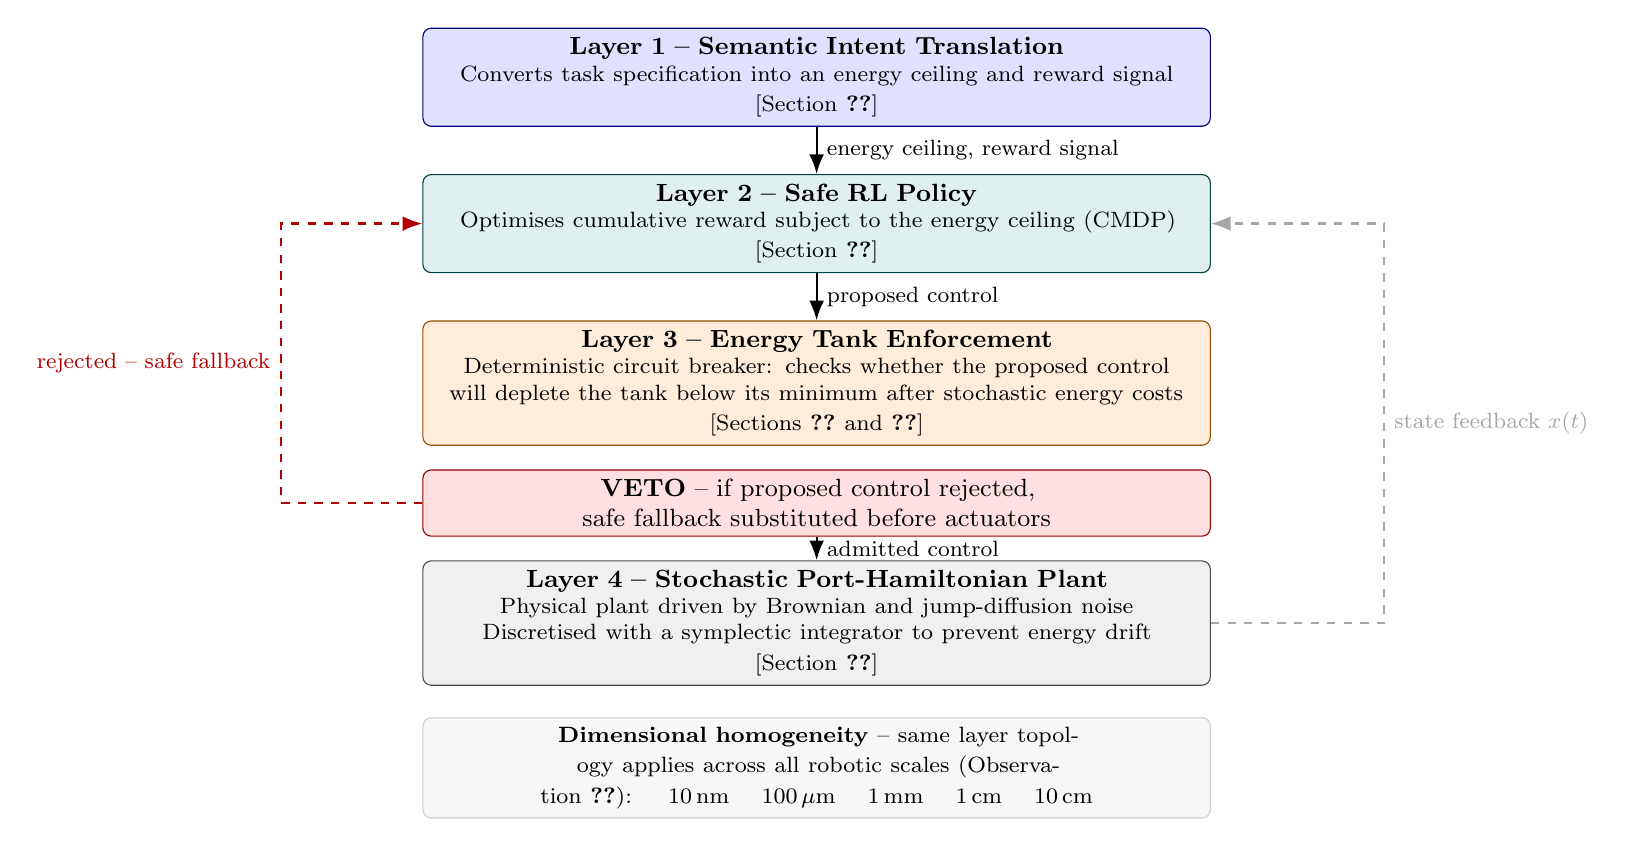
\begin{tikzpicture}[
  every node/.style={font=\small},
  box/.style={draw, rounded corners=3pt, minimum width=10cm, minimum height=1.2cm,
    align=center, text width=9.5cm},
  layer1/.style={box, fill=blue!12, draw=blue!50!black},
  layer2/.style={box, fill=teal!12, draw=teal!50!black},
  layer3/.style={box, fill=orange!15, draw=orange!60!black},
  veto/.style={box, fill=red!12, draw=red!60!black, minimum height=0.8cm},
  layer4/.style={box, fill=gray!12, draw=gray!60!black},
  scalebar/.style={box, fill=gray!6, draw=gray!40, minimum height=0.7cm},
  arr/.style={-{Latex[length=2.5mm]}, thick},
  vetoarr/.style={-{Latex[length=2.5mm]}, dashed, red!70!black, thick},
  fbarr/.style={-{Latex[length=2.5mm]}, dashed, gray!70, thick},
]

\node[layer1] (L1) at (0,0) {%
  \textbf{Layer 1 -- Semantic Intent Translation}\\
  \footnotesize Converts task specification into an energy ceiling and reward signal\\
  \footnotesize [Section~\ref{sec:layer1}]};

\node[layer2, below=0.6cm of L1] (L2) {%
  \textbf{Layer 2 -- Safe RL Policy}\\
  \footnotesize Optimises cumulative reward subject to the energy ceiling (CMDP)\\
  \footnotesize [Section~\ref{sec:layer2}]};

\node[layer3, below=0.6cm of L2] (L3) {%
  \textbf{Layer 3 -- Energy Tank Enforcement}\\
  \footnotesize Deterministic circuit breaker: checks whether the proposed control\\
  \footnotesize will deplete the tank below its minimum after stochastic energy costs\\
  \footnotesize [Sections~\ref{sec:layer3} and \ref{sec:admissibility}]};

\node[veto, below=0.3cm of L3] (VETO) {%
  \textbf{VETO} -- if proposed control rejected, safe fallback substituted before actuators};

\node[layer4, below=0.3cm of VETO] (L4) {%
  \textbf{Layer 4 -- Stochastic Port-Hamiltonian Plant}\\
  \footnotesize Physical plant driven by Brownian and jump-diffusion noise\\
  \footnotesize Discretised with a symplectic integrator to prevent energy drift\\
  \footnotesize [Section~\ref{sec:layer4}]};

\node[scalebar, below=0.4cm of L4] (SC) {%
  \footnotesize \textbf{Dimensional homogeneity} -- same layer topology applies across all
  robotic scales (Observation~\ref{obs:scale}): \quad
  10\,nm \quad 100\,$\mu$m \quad 1\,mm \quad 1\,cm \quad 10\,cm};

\draw[arr] (L1.south) -- node[right,font=\footnotesize]{energy ceiling, reward signal} (L2.north);
\draw[arr] (L2.south) -- node[right,font=\footnotesize]{proposed control} (L3.north);
\draw[arr] (VETO.south) -- node[right,font=\footnotesize]{admitted control} (L4.north);

\draw[vetoarr] (VETO.west) -- ++(-1.8,0) |-
  node[left,font=\footnotesize,pos=0.25]{rejected -- safe fallback} (L2.west);

\draw[fbarr] (L4.east) -- ++(2.2,0) |-
  node[right,font=\footnotesize,pos=0.25]{state feedback $x(t)$} (L2.east);

\end{tikzpicture}%
}% end resizebox
\caption{The EA-HC four-layer architecture. Downward arrows carry the signal flow from
symbolic intent to physical actuation. The red dashed veto path returns a safe fallback
$u_{\mathrm{safe}}$ to Layer~2 whenever the proposed control $u_\pi$ falls outside the
admissible set $\mathcal{U}_{\mathrm{EAHC}}$. The grey dashed arrow carries state feedback
$x(t)$ from Layer~4 back to Layers~2 and 3. The admissibility condition \eqref{eq:admiss}
is dimensionally homogeneous in Joules, enabling the same layer topology to be instantiated
across seven orders of magnitude in operating scale (Observation~\ref{obs:scale}).}
\label{fig:arch}
\end{figure}

\subsection{Layer 1: Semantic Intent Translation}
\label{sec:layer1}

The topmost layer is the entry point for human intent into the architecture. It receives a task
specification -- expressed in natural language, a formal task algebra, or a structured symbolic
representation -- and translates it into two signals that the layers below can act on: a scalar
energy ceiling $E_{\max}\in\mathbb{R}_{>0}$ and a task reward signal $r$. The mapping:
\begin{equation}
\mathcal{M}:\text{TaskSpec}\to(E_{\max},r)
\label{eq:mapping}
\end{equation}
performs a function that has no direct counterpart in standard robot control pipelines. In
most architectures, task specifications influence only the reward or cost function that a planner
optimises; they do not constrain the energy budget of the actuators \cite{kober2013,sutton2018}.
The mapping $\mathcal{M}$ closes this gap by treating task semantics as a source of
thermodynamic information. A task labelled as high-contact (e.g., manipulation against a
stiff environment) receives a higher $E_{\max}$ than a task labelled as proximity-only
(e.g., inspection without tissue contact) \cite{ferraguti2015,haddadin2017}. The physical safety
envelope is therefore not fixed at design time but is adapted continuously to the semantic
content of the current task.

The novelty of Layer~1 lies in the \emph{concept} of treating task-semantic information as a
source of thermodynamic budget constraints -- a composition not present in existing
architectures. In the current implementation, $\mathcal{M}$ is instantiated as a rule-based
lookup informed by the constraint-based task specification framework of Borghesan et al.\
\cite{borghesan2016} and the iTaSC formalism of Vanthienen et al.\ \cite{vanthienen2013}.
These frameworks provide a structured vocabulary for expressing task constraints that can be
systematically associated with energy bounds. The rule-based approach is deliberately
conservative: it is verifiable by inspection and introduces no learned uncertainty into the
safety-critical energy ceiling. The principal limitation -- and the motivation for the LLM-based
extension described in Section~\ref{sec:llm} -- is that the mapping is domain-specific and
requires manual authoring for each new task class. This is acknowledged explicitly in
Section~\ref{sec:sem-limit}.

\subsection{Layer 2: Safe RL Policy}
\label{sec:layer2}

Layer~2 is responsible for generating task-level behaviour within the energy budget supplied
by Layer~1. A Constrained Markov Decision Process (CMDP) policy $\pi$ \cite{altman1999}
operates on the current system state $x$ and the energy ceiling $E_{\max}$, optimising
cumulative reward subject to a long-run energy constraint:
\begin{equation}
\max_\pi\;\mathbb{E}\!\Bigl[\sum_{t=0}^\infty \gamma^t r_t\Bigr]
\quad\text{s.t.}\quad
\mathbb{E}\!\Bigl[\sum_{t=0}^\infty \gamma^t H(x_t)\Bigr]\le E_{\max},
\label{eq:cmdp}
\end{equation}
where $\gamma\in(0,1)$ is the discount factor shared with the reward objective, ensuring the
constraint sum converges and remains dimensionally consistent with $E_{\max}$ in Joules.
The discount factor is necessary: without it, $\sum H(x_t)$ has units of Joules$\times$steps
rather than Joules, and the constraint is ill-posed. The energy ceiling $E_{\max}\in\mathbb{R}_{>0}$
produced by Layer~1 enters \eqref{eq:cmdp} directly as the right-hand side bound,
establishing a consistent energy language from the semantic layer through to the RL policy.

The CMDP formulation was chosen over unconstrained RL because it provides a principled
mechanism for encoding the energy ceiling as a hard constraint on the policy's behaviour over
time, rather than as a soft penalty term in the reward that a sufficiently capable policy might
learn to trade away \cite{garcia2015,achiam2017}. The constraint is expressed in terms of the
Hamiltonian $H(x_t)$, which is the same quantity tracked by the energy tank in Layer~3,
creating a consistent energy language across both layers.

The policy outputs a nominal control $u_\pi$ at each time step, which is forwarded to Layer~3
for admissibility screening before it reaches the actuators. It is important to note that
Layer~2 provides statistical safety in the sense of expected constraint satisfaction over a
trajectory \cite{garcia2015}, but it does not provide a per-step guarantee. A policy that
satisfies \eqref{eq:cmdp} in expectation may still propose controls that are instantaneously
inadmissible from the tank's perspective. This failure mode is well-documented in the safe RL
literature under distributional shift, where the policy encounters states outside its training
distribution and constraint satisfaction is no longer guaranteed \cite{garcia2015,achiam2017}.
Layer~3 exists precisely to intercept such proposals. The state $x(t)$ measured from the plant
feeds back into the policy at every step, closing the loop between physical reality and the
learned behaviour.

\begin{remark}[Consistency between $E_{\max}$ and $T_{\max}$]
\label{rem:consistency}
The energy ceiling $E_{\max}$ produced by Layer~1 enters the discounted CMDP constraint
\eqref{eq:cmdp} as a present-value occupancy-weighted Joule budget. If the Hamiltonian is
pathwise bounded by the tank ceiling, $H(x_t)\le T_{\max}$ for all $t$, then
$\mathbb{E}[\sum_{t=0}^\infty\gamma^t H(x_t)]\le T_{\max}/(1-\gamma)$. For the CMDP
constraint to be satisfiable, a sufficient consistency condition is:
\begin{equation}
T_{\max}\le\frac{E_{\max}}{1-\gamma}.
\label{eq:consist}
\end{equation}
Equivalently, $(1-\gamma)T_{\max}\le E_{\max}$: the per-step marginal energy cost discounted
to present value must not exceed the semantic budget. This condition constrains the system
engineer's choice of $T_{\max}$ given the semantically derived $E_{\max}$ and the RL discount
factor $\gamma$; it should be verified at design time before training the CMDP policy. The
minimum threshold $T_{\min}\in(0,T_{\max})$ provides a safety margin absorbing estimation
errors in $\delta_{\mathrm{It\hat{o}}}$ and $\delta_{\mathrm{L\acute{e}vy}}$.
\end{remark}

\begin{remark}[Relationship between the CMDP constraint and the tank condition]
\label{rem:cmdp-tank}
The CMDP constraint \eqref{eq:cmdp} bounds the cumulative sum of $H(x_t)$ in expectation --
a soft, time-averaged objective that the RL policy learns to respect through training. The tank
admissibility condition \eqref{eq:admiss} is a per-step, hard constraint on the energy flow out
of the tank. The two are not equivalent and do not imply one another: a policy satisfying
\eqref{eq:cmdp} may still propose individual controls $u_\pi$ that violate \eqref{eq:admiss}
on particular time steps, and vice versa. Their roles are complementary: the CMDP reduces the
statistical frequency with which $u_\pi$ falls outside $\mathcal{U}_{\mathrm{EAHC}}$, while
Layer~3 ensures that any such violation is intercepted before reaching the actuators. The
formal composition of these two safety mechanisms -- in particular, whether CMDP feasibility
reduces the worst-case veto rate -- is left as an open problem.
\end{remark}

\subsection{Layer 3: Energy Tank Enforcement}
\label{sec:layer3}

Layer~3 is the deterministic safety core of the EA-HC architecture. It implements the energy
tank originally introduced by Ferraguti et al.\ \cite{ferraguti2013,ferraguti2015,secchi2007}
and extends it with two stochastic energy buffers derived from the It\^{o}--L\'{e}vy formula
(Section~\ref{sec:admissibility}). The layer maintains a scalar energy reservoir $T_t$ that
tracks how much energy remains available for expenditure. At every control cycle, before any
control signal reaches the actuators, Layer~3 evaluates whether the proposed control $u_\pi$
from Layer~2 is admissible: that is, whether executing it would leave the tank above the
minimum threshold $T_{\min}$ after accounting for the power drawn by the control action and
the stochastic energy taxes imposed by the operating environment.

The architectural significance of this layer is that it provides a safety guarantee that is
independent of the quality or correctness of the upstream policy. Even if the CMDP policy in
Layer~2 produces a control that is locally optimal according to its learned value function but
globally inadmissible from an energy standpoint -- whether due to incomplete training,
distributional shift, or simply the inherent imprecision of statistical learning
\cite{garcia2015,achiam2017} -- Layer~3 intercepts that control and substitutes the
minimum-norm passive fallback before any physical harm can occur. This separation between
intent generation (Layer~2) and intent enforcement (Layer~3) parallels the principle of runtime
monitoring in safety-critical systems, where a verified supervisor intercepts unsafe commands
from an unverified controller \cite{pnueli1989,seshia2018}.

The tank state $T_t$ is updated at every time step based on the actual energy consumed by
the admitted control and the stochastic energy injections estimated from the current state. It
is bounded below by $T_{\min}>0$, which is a design parameter set by the system engineer to
provide a safety margin against estimation errors in the stochastic buffers. When the tank
approaches depletion under sustained disturbance, the veto rate increases, which serves as a
system-level signal that the environment is more energetically demanding than the current
policy anticipated \cite{ferraguti2015}. The extended admissibility condition is derived in
detail in Section~\ref{sec:admissibility}.

\subsection{Layer 4: Stochastic Port-Hamiltonian Plant}
\label{sec:layer4}

Layer~4 is the physical plant: the robotic system whose dynamics the architecture is designed
to control safely. Within the EA-HC framework, the plant is modelled as an SPHS \eqref{eq:sphs},
which extends the deterministic pH formulation of Section~\ref{sec:prelim} with both continuous
Brownian diffusion and discrete jump events. This modelling choice is a deliberate commitment
about which physical phenomena the safety architecture takes responsibility for. The Brownian
term $\sigma(x)\,dW_t$ captures diffusive disturbances such as thermal noise, sensor jitter,
and unmodelled friction that are continuous in time \cite{gardiner1985,jazwinski1970}. The jump
term $\int_{\mathcal{Z}}\gamma(x,z)\tilde{N}(dt,dz)$ captures episodic impulsive events such
as collisions, sudden load changes, or, in the microrobotics context, pressure impulses from
pulsatile blood flow \cite{applebaum2009,ku1997}.

Both noise sources enter the system through the port structure of the pH model -- they are
intrinsic to the plant's operating environment rather than exogenous inputs from outside the
system boundary \cite{vanderschaft1995,cordoni2022}. This is the precise sense in which the
scope of the thermodynamic veto is bounded: Layer~3 accounts for the energy injected by these
port-connected disturbances, but it does not account for forces that act on the robot without
passing through the pH port (e.g., a river current pushing a passive body). The distinction is
discussed in detail in the limitations (Section~\ref{sec:drift}).

The admitted control $u_{\mathrm{adm}}$ from Layer~3 drives the plant through the input
matrix $g(x)$. The resulting state $x(t)$ is measured and fed back to both Layer~2 (where
it updates the policy's state estimate) and Layer~3 (where it updates the tank's energy
accounting and the stochastic buffer estimates for the next cycle). This feedback closes the
loop and allows the architecture to adapt continuously to the evolving energy landscape of the
physical system. The digital implementation of this feedback loop uses the symplectic
Euler--Maruyama scheme described in Section~\ref{sec:symplectic}, which preserves the
Hamiltonian structure of the continuous-time model and prevents the artificial energy drift that
would otherwise corrupt the tank's energy ledger.

\subsection{Extended Admissibility Condition}
\label{sec:admissibility}

The admissibility condition screens whether the proposed control $u_\pi$ is safe to admit.
Applying the It\^{o}--L\'{e}vy formula \eqref{eq:ito-levy} to the Hamiltonian $H$ along
trajectories of \eqref{eq:sphs}, the expected energy injected by stochastic disturbances over
one control interval $\Delta t$ decomposes into two buffers.

\paragraph{It\^{o} buffer.} The continuous Brownian contribution, following the infinitesimal
generator analysis of Cordoni et al.\ \cite{cordoni2022}:
\begin{equation}
\delta_{\mathrm{It\hat{o}}} =
\tfrac{1}{2}\operatorname{tr}\!\bigl[\sigma(x)^T\nabla^2 H(x)\,\sigma(x)\bigr]\cdot\Delta t.
\label{eq:ito-buf}
\end{equation}

\paragraph{L\'{e}vy buffer.} Under Assumption~\ref{ass:struct} (S1)--(S3), jump events displace
momenta only: $\gamma=(0,\gamma_p(z))$. The second-order Taylor remainder of $H$ with respect
to a momentum-only displacement reduces exactly (with no approximation, since $K$ is
quadratic in $p$):
\begin{equation}
H(x+\gamma)-H(x)-\nabla H^T\gamma
= K(p+\gamma_p)-K(p)-\nabla_p K^T\gamma_p
= \frac{\|\gamma_p(z)\|^2}{2m}\ge 0.
\label{eq:taylor-exact}
\end{equation}
The non-negativity holds unconditionally -- no convexity of $V(q)$ is required -- because
$V(q)$ drops out entirely from the $p$-Taylor expansion. Integrating against $\nu$ over one
control interval $\Delta t$:
\begin{equation}
\delta_{\mathrm{L\acute{e}vy}} = \Delta t\int_{\mathcal{Z}}\frac{\|\gamma_p(z)\|^2}{2m}\,\nu(dz)\ge 0.
\label{eq:levy-buf}
\end{equation}
The finite-second-moment condition (S4) ensures $\delta_{\mathrm{L\acute{e}vy}}<\infty$.
The result in \eqref{eq:taylor-exact}--\eqref{eq:levy-buf} is exact under
Assumption~\ref{ass:struct}; no small-jump approximation is required.

\paragraph{Admissibility condition.} The total energy extracted from the tank over one control
interval $\Delta t$ has two components: the deterministic power drawn by the admitted control,
$y^T u_\pi\,\Delta t=\nabla H(x)^T g(x)u_\pi\,\Delta t$, and the stochastic energy injected by
the noise, $\delta_{\mathrm{It\hat{o}}}+\delta_{\mathrm{L\acute{e}vy}}$. A control $u_\pi$
is admitted if and only if the tank level $T$ remains above the minimum threshold after both
deductions:
\begin{equation}
\mathcal{U}_{\mathrm{EAHC}} = \Bigl\{u_\pi \;\Big|\;
  T - \nabla H(x)^T g(x)\,u_\pi\,\Delta t
  - \bigl(\delta_{\mathrm{It\hat{o}}}+\delta_{\mathrm{L\acute{e}vy}}\bigr)\ge T_{\min}\Bigr\}.
\label{eq:admiss}
\end{equation}
The set $\mathcal{U}_{\mathrm{EAHC}}$ is a half-space in $u_\pi$ (for fixed $x$ and $T$), so
the minimum-norm element satisfying \eqref{eq:admiss} exists and is unique whenever the set
is non-empty \cite{ferraguti2013}. If $u_\pi\notin\mathcal{U}_{\mathrm{EAHC}}$, Layer~3
substitutes the minimum-norm passive fallback
$u_{\mathrm{safe}}=\arg\min\|u\|$ subject to \eqref{eq:admiss}, which reduces to
$u_{\mathrm{safe}}=0$ when $T-\delta_{\mathrm{It\hat{o}}}-\delta_{\mathrm{L\acute{e}vy}}<T_{\min}$
regardless of $u_\pi$ -- i.e., when the stochastic debits alone would deplete the tank, no
control action is admissible and the robot is immobilised until the tank recharges. When
$\nabla H(x)^T g(x)=0$ (i.e., at energy extrema such as equilibria of regulation tasks), the
power-flow term vanishes and the admissibility condition reduces to the pure stochastic
constraint $T-\delta_{\mathrm{It\hat{o}}}-\delta_{\mathrm{L\acute{e}vy}}\ge T_{\min}$,
independent of $u_\pi$; in this case any control is equally (in)admissible and the fallback is
$u_{\mathrm{safe}}=0$. The stochastic buffers and the power-flow term together account for all
energy leaving the tank; no exogenous non-port terms are included, in keeping with the bounded
scope of the thermodynamic veto.

\subsection{Symplectic Euler--Maruyama Discretization}
\label{sec:symplectic}

For digital implementation, the SPHS \eqref{eq:sphs} is discretized using the symplectic
Euler--Maruyama scheme \cite{milstein1995,leimkuhler2004}:
\begin{equation}
\begin{aligned}
p_{k+1} &= p_k - \nabla_q H(q_k, p_{k+1})\,\Delta t
           + g_p(x_k)u_k\,\Delta t + \sigma_p(x_k)\,\Delta W_k,\\
q_{k+1} &= q_k + \nabla_p H(q_k, p_{k+1})\,\Delta t,
\end{aligned}
\label{eq:sym-EM}
\end{equation}
where $(q,p)$ are generalized coordinates and momenta, and $\Delta W_k\sim\mathcal{N}(0,\Delta t\,)$.

\paragraph{Implicit step resolution.} The momentum update in \eqref{eq:sym-EM} is implicit in
$p_{k+1}$ through $\nabla_q H(q_k,p_{k+1})$. For the separable Hamiltonian
$H=K(p)+V(q)$ of Assumption~\ref{ass:struct}(S1), $\nabla_q H=\nabla_q V(q_k)$ is
independent of $p_{k+1}$, so the implicit step reduces to an \emph{explicit} update:
\begin{equation}
p_{k+1} = p_k - \nabla_q V(q_k)\,\Delta t + g_p(x_k)u_k\,\Delta t + \sigma_p(x_k)\,\Delta W_k.
\end{equation}
No Newton iteration or fixed-point solve is required for any instantiation satisfying
Assumption~\ref{ass:struct}(S1). For non-separable Hamiltonians, the implicit step must be
resolved by a fixed-point iteration or linearization; this should be verified for each new
instantiation.

\paragraph{Structural validity.} Stochastic symplecticity in the mean-square sense holds for
separable Hamiltonians $H=K(p)+V(q)$ with additive noise on $p$ only \cite{milstein2002} --
the setting of the microrobotics instantiation (Section~\ref{sec:micro}). For state-dependent
(multiplicative) $\sigma$, fully implicit schemes are required \cite{milstein2003}. For the
jump term, symplecticity requires the jump map $x\mapsto x+\gamma(x,z)$ to be symplectic;
this holds for momentum-only jumps $\gamma=(0,\gamma_p)$ under Assumption~\ref{ass:struct}(S3)
(Jacobian $=I$, so $dq\wedge dp$ is preserved), but not generically. These assumptions are
satisfied in the microrobotics case study and should be verified for other instantiations.

The symplectic structure preserves the Poincar\'{e} invariants of the Hamiltonian flow up to
discretization error of order $\mathcal{O}(\Delta t^2)$ \cite{leimkuhler2004}, preventing
artificial energy drift that would contaminate the tank's energy accounting.

\section{Theoretical Analysis}
\label{sec:theory}

\subsection{Compositional Passivity}

\begin{proposition}[Compositional Passivity]
\label{prop:passivity}
Consider the EA-HC stack with plant \eqref{eq:sphs}, tank dynamics \eqref{eq:tank}, and
admissibility condition \eqref{eq:admiss}. If at every time step the admitted control satisfies
$u_{\mathrm{adm}}\in\mathcal{U}_{\mathrm{EAHC}}$, then the closed-loop system is passive with
supply rate $s(u,y)=y^Tu$ in expectation:
\begin{equation}
\mathbb{E}[H(x(t))] \le H(x(0)) + \int_0^t \mathbb{E}[y(s)^T u_{\mathrm{adm}}(s)]\,ds.
\label{eq:passivity}
\end{equation}
\end{proposition}

\begin{proof}
\textbf{Step 1: Non-explosion and localization.} Under Assumption~\ref{ass:struct} and global
linear growth of the coefficients $[J-R,\,g,\,\sigma_p,\,\gamma_p]$, the SDE \eqref{eq:sphs}
admits a unique global c\`{a}dl\`{a}g strong solution with $\tau_\infty=\infty$ a.s.\
\cite{applebaum2009,khasminskii2012}. Define stopping times
$\tau_n=\inf\{t\ge 0:H(x(t))\ge n\}$ for $n\in\mathbb{N}$. Since $H(x_0)\le E_{\max}<\infty$
and the solution is non-explosive, $\tau_n\nearrow\infty$ a.s.\ by Applebaum
\cite{applebaum2009} (Theorem~6.2.3). On the stopped interval $[0,\tau_n]$, the Hamiltonian
is bounded by $n$, so the square-integrability condition
$\int_{\mathcal{Z}}\mathbb{E}[(H(x^{\tau_n}+\gamma)-H(x^{\tau_n}))^2]\nu(dz)<\infty$
holds under (S4), and the compensated Poisson integral is a square-integrable martingale
(Applebaum \cite{applebaum2009}, Proposition~4.4.1). The stochastic passivity in expectation
framework of Lanchares and Haddad \cite{lanchares2023} establishes the equivalence between
the energy-function inequality and the supermartingale property for It\^{o} diffusions; we
extend this to the jump-diffusion case via the It\^{o}--L\'{e}vy formula following the same
argument.

\textbf{Step 2: Per-step discrete inequality.} At each Euler--Maruyama step $k$ on the stopped
trajectory, applying the It\^{o}--L\'{e}vy formula \eqref{eq:ito-levy} to $H$ and using
Assumption~\ref{ass:struct}(S1)--(S3):
\begin{equation}
\mathbb{E}[H(x_{k+1}^{\tau_n})]-\mathbb{E}[H(x_k^{\tau_n})]
\le \Delta t\,\mathbb{E}[\nabla H^T g\,u_{\mathrm{adm},k}]
+ \mathbb{E}[\delta_{\mathrm{It\hat{o}}}]
+ \mathbb{E}[\delta_{\mathrm{L\acute{e}vy}}],
\label{eq:perstep}
\end{equation}
where the Brownian increment $\nabla H^T\sigma_p\Delta W_k$ and the compensated Poisson
increment $\int[H(x+\gamma)-H(x)]\tilde{N}(\Delta t,dz)$ have zero expectation by the
martingale property of Step~1. The admissibility condition \eqref{eq:admiss} ensures the tank
absorbs $\delta_{\mathrm{It\hat{o}}}+\delta_{\mathrm{L\acute{e}vy}}$ per step before releasing net
power $\nabla H^T g\,u_{\mathrm{adm},k}\,\Delta t$; formally, the tank balance at step $k$ gives
$\nabla H^T g\,u_{\mathrm{adm},k}\,\Delta t+\delta_{\mathrm{It\hat{o}}}+\delta_{\mathrm{L\acute{e}vy}}
\le T_k-T_{\min}$, so the right-hand side of \eqref{eq:perstep} is bounded by the external
supply $\Delta t\,\mathbb{E}[y_k^T u_{\mathrm{adm},k}]$.

\textbf{Step 3: Summation and limit.} Summing \eqref{eq:perstep} over $k=0,\ldots,\lfloor t/\Delta t\rfloor-1$:
\[
\mathbb{E}[H(x^{\tau_n}(t))]\le H(x_0)+\sum_k \Delta t\,\mathbb{E}[y_k^T u_{\mathrm{adm},k}].
\]
As $\Delta t\to 0$ the Riemann sum converges to
$\int_0^t\mathbb{E}[y(s)^T u_{\mathrm{adm}}(s)]\,ds$ under standard integrability of
$u_{\mathrm{adm}}$. Taking $n\to\infty$ and applying the monotone convergence theorem
(since $H\ge 0$ and $\tau_n\nearrow\infty$ a.s.) yields \eqref{eq:passivity}.
\end{proof}

\subsection{Stochastic Safety Guarantee}

\begin{proposition}[Stochastic Energy Bound]
\label{prop:safety}
Under the conditions of Proposition~\ref{prop:passivity} -- specifically: (i) the admissibility
condition \eqref{eq:admiss} is enforced at every discrete time step; (ii) Assumption~\ref{ass:struct}
holds; (iii) the plant model $H(x)$ is faithful to the true system; and (iv) the CMDP policy
$\pi$ has converged to satisfy constraint \eqref{eq:cmdp} -- if $T_0\ge T_{\min}$ and
$H(x_0)\le E_{\max}$, and the admitted control satisfies
$\|u_{\mathrm{adm}}(t)\|\le u_{\max}<\infty$ for all $t\ge 0$, then for all $t\in[0,\mathcal{T}]$:
\begin{equation}
\Pr\bigl[H(x(t))>E_{\max}\bigr]
\le \frac{H(x_0)+u_{\max}\cdot\|g\|_\infty\cdot\|\nabla H\|_\infty\cdot\mathcal{T}}{E_{\max}}.
\label{eq:safety}
\end{equation}
\end{proposition}

\begin{proof}
The boundedness assumption $\|u_{\mathrm{adm}}\|\le u_{\max}$ ensures that the supply-rate
integral satisfies $\int_0^\mathcal{T}\mathbb{E}[y(s)^T u_{\mathrm{adm}}(s)]\,ds
\le u_{\max}\cdot\|g\|_\infty\cdot\|\nabla H\|_\infty\cdot\mathcal{T}<\infty$. Apply
Markov's inequality \cite{billingsley1995} to \eqref{eq:passivity} with $V=H\ge 0$ to obtain
\eqref{eq:safety}. The bound is finite-horizon and conservative: it ignores the variance of
$H$ and the tail structure of the L\'{e}vy noise. Tighter bounds via the L\'{e}vy exponent
(Cram\'{e}r--Chernoff) are available \cite{applebaum2009} and are identified as a direction
for future work.
\end{proof}

\subsection{Dimensional Homogeneity and Scale-Agnostic Formulation}

\begin{observation}[Dimensional Homogeneity]
\label{obs:scale}
The admissibility condition \eqref{eq:admiss} is dimensionally homogeneous in energy units
(Joules) and is independent of the absolute magnitude of the system coordinates.
Consequently, the same EA-HC layer topology applies to robotic systems across arbitrary
operating scales, provided the Hamiltonian $H$ and diffusion coefficients $\sigma$ are
specified consistently with the system's energy domain \cite{vanderschaft2014,goldstein2002}.
\end{observation}

\begin{proof}
The tank level $T$, the buffers $\delta_{\mathrm{It\hat{o}}}$ and
$\delta_{\mathrm{L\acute{e}vy}}$, and the minimum threshold $T_{\min}$ are all measured in
Joules. The admissibility condition \eqref{eq:admiss} is a scalar inequality in energy, with no
explicit dependence on length, mass, or time scales \cite{vanderschaft2014}. The same
inequality therefore applies verbatim at any scale; only the numerical values of $H$, $\sigma$,
and $\nu$ change. This is a dimensional consistency observation: a formal invariance theorem
under a specified nondimensionalization group would require additional assumptions on the
scaling of $H$, $\sigma$, and $\nu$ across the macro-to-micro range and is left as future work.
\end{proof}

\section{Medical Microrobotics: Extreme-Case Instantiation}
\label{sec:micro}

Medical microrobotics represents an extreme-case instantiation of the EA-HC framework:
operating scales span from centimeters (catheter-tipped robots \cite{sitti2018}) to nanometers
(DNA-origami walkers \cite{douglas2009}), thermal noise dominates actuation forces below
roughly 10\,$\mu$m \cite{purcell1977}, and the operating environment (blood, interstitial fluid,
cerebrospinal fluid) imposes both stochastic Brownian disturbances and episodic jump-like
perturbations from pulsatile flow.

\subsection{SPHS Instantiation for Microswimmers}

A magnetic microswimmer is modeled as a rigid body with generalized coordinates
$q=(p_x,p_y,p_z,\varphi)^T$ (position and orientation) and momenta $p=m\dot{q}$. The
Hamiltonian is:
\begin{equation}
H(q,p) = \frac{1}{2m}\|p\|^2 + V_{\mathrm{mag}}(q),
\label{eq:micro-H}
\end{equation}
where $V_{\mathrm{mag}}$ is the magnetic potential energy from the external actuation coils
\cite{sitti2018}. The diffusion coefficient is set by the fluctuation-dissipation theorem
\cite{einstein1905}:
\begin{equation}
\sigma = \sqrt{2k_B T_{\mathrm{env}}\,\zeta}\,I,
\label{eq:sigma}
\end{equation}
where $k_B$ is Boltzmann's constant, $T_{\mathrm{env}}$ is the fluid temperature, and $\zeta$
is the drag coefficient from Stokes' law. Jump events $\gamma(x,z)$ model pulsatile pressure
impulses with L\'{e}vy intensity $\nu$ calibrated from physiological data \cite{ku1997}.
Assumption~\ref{ass:struct}(S1)--(S4) is satisfied: the Hamiltonian \eqref{eq:micro-H} is
separable, the diffusion \eqref{eq:sigma} acts on momenta only, pulsatile impulses displace
momenta only, and the finite-second-moment condition holds for physiologically calibrated
$\nu$ \cite{ku1997}.

\subsection{Buffer Evaluation at the Microscale}

Substituting \eqref{eq:micro-H} into \eqref{eq:ito-buf} with the diffusion coefficient
\eqref{eq:sigma} and using $\nabla^2 H=\frac{1}{m}I$ (from the quadratic kinetic energy term)
yields the It\^{o} buffer directly:
\begin{equation}
\delta_{\mathrm{It\hat{o}}} = \frac{k_B T_{\mathrm{env}}\,\zeta}{m}\cdot n\cdot\Delta t,
\label{eq:ito-micro}
\end{equation}
where $n$ is the state dimension.

For the L\'{e}vy buffer, under Assumption~\ref{ass:struct}(S1)--(S3), pulsatile pressure
impulses displace the swimmer's momentum only: $\gamma(x,z)=(0,\gamma_p(z))$ with
$\gamma_p(z)=z$. By \eqref{eq:taylor-exact} the second-order remainder is exactly
$\|z\|^2/(2m)$, so:
\begin{equation}
\delta_{\mathrm{L\acute{e}vy}} = \Delta t\int_0^\infty\frac{\|z\|^2}{2m}\,\nu(dz).
\label{eq:levy-micro}
\end{equation}
This result is exact under Assumption~\ref{ass:struct} -- no approximation is invoked.

Both $\delta_{\mathrm{It\hat{o}}}$ and $\delta_{\mathrm{L\acute{e}vy}}$ are computable from
known physical constants and calibrated physiological parameters \cite{ku1997}, confirming
that the admissibility condition \eqref{eq:admiss} is evaluable at the microscale. The
tightness of these bounds -- i.e., whether they are conservative or near-exact in practice --
will be assessed in forthcoming simulation studies.

\subsection{Scale Comparison}

Table~\ref{tab:scale} summarizes the EA-HC instantiation across five robotic embodiments
spanning seven orders of magnitude in characteristic length.

\begin{table}[t]
\centering
\caption{Scale-agnostic instantiation of the EA-HC architecture.
$^\dagger$At 10\,nm quantum effects become non-negligible and the classical SPHS Hamiltonian
assumption may break; this row is conjectural and included for illustrative completeness only.}
\label{tab:scale}
\begin{tabular}{lllll}
\toprule
System & Scale & $H$ domain & $\sigma$ origin & Jump source\\
\midrule
Surgical robot    & 10\,cm & Rigid-body KE & Encoder noise    & Tool contact\\
Soft exoskeleton  & 1\,cm  & Elastic PE    & Gait variability & Stumble events\\
Catheter robot    & 1\,mm  & Bending energy& Blood drag       & Pulsatile flow\\
Microswimmer      & 100\,$\mu$m & Thermal KE & FDT (Eq.~\ref{eq:sigma}) & Pulse impulse\\
DNA nanobot$^\dagger$ & 10\,nm & Binding energy & Thermal agitation & Molecular collision\\
\bottomrule
\end{tabular}
\end{table}

\section{Discussion}
\label{sec:discussion}

\subsection{Architectural Significance}

The EA-HC framework is, to our knowledge, the first architecture to integrate all four layers
(semantic intent, safe RL, energy tank enforcement, and stochastic pH plant) into a single
closed stack. Each layer has antecedents in the literature \cite{ferraguti2013,altman1999,cordoni2022,borghesan2016};
the contribution is the vertical integration and the explicit interface definitions between layers.

The Handshake Gap is not a gap in mathematics but a gap in architecture. Energy-aware
controllers exist \cite{ferraguti2015,schindlbeck2015}; safe RL methods exist
\cite{garcia2015,achiam2017}; stochastic pH models exist \cite{cordoni2022,fang2017}. What
has been missing is a load-bearing interface between them that allows a symbolic task
specification to flow downward as a thermodynamic budget and a passivity certificate to flow
upward as a safety guarantee. The mapping $\mathcal{M}$ (Layer~1 to Layer~2) and the
admissibility condition (Layer~2 to Layer~3) are the two novel interfaces that close this gap.

\subsection{Structural vs.\ Statistical Safety Enforcement}

Unlike traditional Safe RL frameworks that rely on a CMDP to learn safety boundaries
statistically, the EA-HC architecture enforces safety structurally. The Handshake Gap is
fundamentally a language barrier: high-level agents operate in symbolic rewards, while physical
systems operate in Joules. By establishing energy as the universal currency, the EA-HC
provides a deterministic circuit breaker. Even if an RL policy produces a nominally optimal
trajectory that is physically destructive, the Layer~3 energy tank acts as a final arbiter,
ensuring that passivity cannot be violated by the admitted control.

This distinction matters for certification. Statistical safety (CMDP) provides bounds on
expected constraint violation but cannot rule out individual catastrophic episodes
\cite{garcia2015}. Structural safety (the energy veto) provides a hard guarantee per control
cycle, conditional on model fidelity (see Section~\ref{sec:model-cond}), and is therefore
closer in spirit to the deterministic safety certificates sought by standards such as IEC~61508
and ISO~10218 for safety-critical robotic systems \cite{seshia2018}. The two mechanisms are
complementary: the CMDP reduces the frequency with which Layer~3 must veto, while Layer~3
ensures that any veto failure at the CMDP level does not propagate to the actuators.

\subsection{Applications Across Robotic Domains}

The dimensional homogeneity of the admissibility condition (Observation~\ref{obs:scale})
implies that the EA-HC architecture is deployable, with appropriate Hamiltonian and diffusion
parameterization, across a wide range of robotic embodiments. Prospective application domains
include legged locomotion \cite{hutter2016}, soft exoskeletons \cite{menguc2013}, aerial
robotics \cite{faessler2018}, underwater vehicles \cite{fossen1994}, space robotics
\cite{flores2014}, and agricultural robotics \cite{bac2014}. In each case, the core safety
substrate (Layers~3--4) remains unchanged; only the Hamiltonian, diffusion model, and
semantic mapping (Layer~1) are domain-specific.

\subsection{Digital Twins and Real-Time Model Updates}

A natural extension of the EA-HC framework is to replace the fixed plant model in Layer~4
with a digital twin that is updated in real time from sensor feedback \cite{grieves2017,tao2019}.
This would allow the admissibility condition to track changes in the system's energy landscape
(e.g., tissue stiffness changes during a surgical procedure \cite{haddadin2017}) and adjust the
stochastic buffers accordingly. Physics-Informed Neural Networks (PINNs) \cite{raissi2019}
offer a promising mechanism for online Hamiltonian identification without requiring explicit
physical models.

\subsection{Semantic Perception and LLM Integration}
\label{sec:llm}

The current implementation of the semantic mapping $\mathcal{M}$ is rule-based. A natural
extension is to leverage large language models (LLMs) to parse nuanced task specifications
(e.g., ``exercise extreme caution near the aortic valve'') and translate them into graded
energy ceilings $E_{\max}$. Recent work on LLM-based task planning for robotics \cite{ahn2023}
provides a foundation for this integration, though the mapping from linguistic hedges to energy
bounds remains an open research problem.

\subsection{Swarm and Quantum Extensions}

For multi-agent microrobot swarms, the EA-HC admissibility condition extends naturally to a
sum of per-agent tank levels, with a global passivity constraint enforced at the swarm
coordinator \cite{vanderschaft2014,wang2017}. At the quantum scale (below 10\,nm), the
classical Hamiltonian $H$ must be replaced by the expectation of the quantum Hamiltonian
operator $\hat{H}$, and the It\^{o} calculus must be replaced by its quantum analogue
\cite{hudson1984}. These extensions are identified as long-horizon research directions.

\subsection{Limitations}

\subsubsection{The Passive Drift Problem}
\label{sec:drift}

A primary limitation of the current thermodynamic focus is what we term \emph{geometric
blindness}. While the EA-HC ensures internal passivity (preventing the robot from becoming
mechanically unstable through its own actuator actions), it does not guarantee spatial survival.
A robot can be perfectly passive and yet be pushed into a vessel wall by exogenous ambient
forces, such as pulsatile blood flow or pressure gradients \cite{nelson2010,ku1997}. In this
iteration, we have deliberately excluded exogenous drift terms to preserve the mathematical
purity of the It\^{o}--L\'{e}vy energy ledger \cite{applebaum2009}, recognizing that spatial
confinement is a distinct safety objective from passivity enforcement, and one properly
addressed by Control Barrier Functions \cite{ames2017}.

\subsubsection{Model-Conditional Determinism and the Sensing-Safety Paradox}
\label{sec:model-cond}

The safety veto is deterministic in its decision logic but remains conditional on the fidelity
of the plant model $H(x)$. If the Hamiltonian or input matrices are misspecified, the energy
tank may track a phantom energy level that does not reflect the true physical state \cite{ljung1999}.
Furthermore, attempting to model every external force introduces a sensing-safety paradox:
the deterministic guarantee becomes vulnerable to fallible environmental sensing (e.g., sensor
occlusion or calibration drift \cite{thrun2005}). The framework trades exhaustive modeling for
mathematical rigor by explicitly bounding the scope of the veto rather than attempting to
account for all possible perturbations.

\subsubsection{Computational Latency}

The real-time evaluation of the two stochastic integrals ($\delta_{\mathrm{It\hat{o}}}$ and
$\delta_{\mathrm{L\acute{e}vy}}$) at high control frequencies (kHz) introduces non-trivial
computational overhead \cite{diehl2009}. Any latency in the veto calculation creates a temporal
safety gap: the robot is briefly unshielded between the intent generation and the energy
admissibility check. Efficient approximations of the L\'{e}vy integral \eqref{eq:levy-buf}
(e.g., via moment matching \cite{cont2006} or sparse quadrature \cite{gerstner1998}) are a
necessary direction for practical deployment.

\subsubsection{Absence of Numerical Simulation}

The current work is a theoretical architecture paper. No numerical simulations or hardware
experiments are reported. The buffer expressions \eqref{eq:ito-micro} and \eqref{eq:levy-micro}
are derived analytically and are evaluable from known physical constants, but their practical
tightness (i.e., whether they are conservative or tight energy bounds) has not been tested.
Simulation studies using the symplectic Euler--Maruyama scheme \eqref{eq:sym-EM} are in
progress and will be reported in a subsequent version.

\subsubsection{CMDP Policy Convergence}

Layer~2 assumes access to a converged CMDP policy $\pi$ satisfying the energy constraint
\eqref{eq:cmdp}. In practice, RL training may produce policies that violate the constraint
during exploration, increasing the frequency of Layer~3 vetoes \cite{garcia2015,achiam2017}.
The interaction between CMDP training dynamics and the energy tank's veto rate is an open
problem.

\subsubsection{Semantic Mapping Fidelity}
\label{sec:sem-limit}

The mapping $\mathcal{M}$ from symbolic task specifications to energy ceilings
(Section~\ref{sec:layer1}) is currently rule-based and domain-specific. Its correctness is not
formally verified: an incorrectly specified $E_{\max}$ (too high or too low) will propagate
through the entire stack. Formal methods for verifying the semantic layer against physical
constraints \cite{pnueli1989,seshia2018} remain an open problem and represent a natural
direction for future work.

\subsubsection{Jump Intensity Calibration}

The L\'{e}vy intensity $\nu$ in \eqref{eq:levy-buf} must be calibrated from physiological or
environmental data \cite{cont2004,ku1997}. Miscalibration of $\nu$ will cause the
$\delta_{\mathrm{L\acute{e}vy}}$ buffer to be either overly conservative (leading to
unnecessary vetoes) or insufficiently cautious (allowing energy violations during rare large
jumps). Online calibration of $\nu$ from streaming sensor data, using e.g.\ sequential Monte
Carlo methods \cite{doucet2001}, is a necessary engineering challenge.

\subsubsection{Tank Depletion Under Sustained Disturbance}

If the stochastic disturbances are sustained over a long horizon, the cumulative buffers
$\delta_{\mathrm{It\hat{o}}}+\delta_{\mathrm{L\acute{e}vy}}$ may deplete the tank even in the
absence of any control action. In this regime, Layer~3 would be forced to veto all actions
(safe fallback $u_{\mathrm{safe}}=0$), effectively immobilizing the robot. A tank replenishment
strategy (e.g., via energy harvesting or planned passive phases) is required for sustained
operation.

\section{Conclusion and Future Work}
\label{sec:conclusion}

This paper has proposed the EA-HC framework as a four-layer architecture for resolving the
Handshake Gap between symbolic task intent and physical safety in robotics. The key
architectural insight is that energy is the universal currency bridging these two levels: a
symbolic task specification can be translated into a thermodynamic budget, and passivity can
be enforced deterministically through an energy veto derived directly from the It\^{o}--L\'{e}vy
formula.

The main theoretical contributions are: (1) the extension of the finite-dimensional SPHS
formulation to the jump-diffusion regime (Section~\ref{sec:prelim}); (2) the extension of the
port-Hamiltonian energy tank admissibility condition by two stochastic buffers
($\delta_{\mathrm{It\hat{o}}}$ and $\delta_{\mathrm{L\acute{e}vy}}$); (3) the Compositional
Passivity and Stochastic Safety propositions establishing closed-loop energy bounds; and (4)
the dimensional homogeneity observation showing that the architecture applies across seven
orders of magnitude in robotic operating scale.

Medical microrobotics serves as an extreme-case instantiation, showing that the architecture
remains evaluable and physically meaningful in Brownian-dominated, jump-diffusion environments.

\paragraph{Future Work.} Future research will focus on three key expansions:
\begin{enumerate}
\item \textbf{Geometric integration via CBF layer.} We intend to integrate a Control Barrier
  Function (CBF) layer \cite{ames2017} to provide geometric guardrails that complement the
  thermodynamic circuit breaker, directly addressing the passive drift problem
  (Section~\ref{sec:drift}). The CBF layer would enforce forward invariance of a spatial safe
  set (e.g., vessel lumen) against exogenous ambient forces, while the EA-HC Layer~3
  continues to enforce thermodynamic passivity. The two layers address orthogonal safety
  objectives and are designed to compose without conflict.

\item \textbf{Semantic mapping via large language models.} To refine Layer~1, we propose
  using LLMs to translate nuanced surgical or operational instructions (e.g., ``exercise
  extreme caution near the aortic valve'') into precise, real-time energy ceilings $E_{\max}$,
  grounding the semantic layer in natural language understanding \cite{ahn2023}.

\item \textbf{Physics-informed model identification.} To mitigate model-conditional risks
  (Section~\ref{sec:model-cond}), we will explore the use of Physics-Informed Neural Networks
  (PINNs) \cite{raissi2019} to learn and update the system Hamiltonian $H(x)$ during live
  deployment, enabling the admissibility condition to track the true energy landscape of a
  time-varying plant.
\end{enumerate}

\bibliographystyle{plainnat}
\begin{thebibliography}{99}

\bibitem{kober2013}
J. Kober, J. A. Bagnell, and J. Peters,
``Reinforcement learning in robotics: A survey,''
\emph{Int. J. Robot. Res.}, vol.~32, no.~11, pp.~1238--1274, 2013.
\url{https://doi.org/10.1177/0278364913495721}

\bibitem{levine2016}
S. Levine, C. Finn, T. Darrell, and P. Abbeel,
``End-to-end training of deep visuomotor policies,''
\emph{J. Mach. Learn. Res.}, vol.~17, no.~39, pp.~1--40, 2016.
\url{https://arxiv.org/abs/1504.00702}

\bibitem{vanderschaft2014}
A. van der Schaft,
\emph{$L_2$-Gain and Passivity Techniques in Nonlinear Control}, 3rd ed.
Springer, 2014.
\url{https://doi.org/10.1007/978-3-319-49992-5}

\bibitem{ferraguti2013}
F. Ferraguti, C. Secchi, and C. Fantuzzi,
``A tank-based approach to impedance control with variable stiffness,''
in \emph{Proc. IEEE ICRA}, 2013, pp.~4948--4953.
\url{https://doi.org/10.1109/ICRA.2013.6631284}

\bibitem{ferraguti2015}
F. Ferraguti, N. Preda, A. Manurung, M. Bonfe, O. Lambercy, R. Gassert,
R. Muradore, P. Fiorini, and C. Secchi,
``An energy tank-based interactive control architecture for autonomous and
teleoperated robotic surgery,''
\emph{IEEE Trans. Robot.}, vol.~31, no.~5, pp.~1073--1088, 2015.
\url{https://doi.org/10.1109/TRO.2015.2455791}

\bibitem{garcia2015}
J. Garc\'{i}a and F. Fern\'{a}ndez,
``A comprehensive survey on safe reinforcement learning,''
\emph{J. Mach. Learn. Res.}, vol.~16, pp.~1437--1480, 2015.
\url{https://jmlr.org/papers/v16/garcia15a.html}

\bibitem{altman1999}
E. Altman,
\emph{Constrained Markov Decision Processes}.
Chapman and Hall/CRC, 1999.
\url{https://doi.org/10.1201/9781315140223}

\bibitem{vanderschaft1995}
A. van der Schaft and B. Maschke,
``The Hamiltonian formulation of energy conserving physical systems with
external ports,''
\emph{Arch. Elektron. \"{U}bertrag.}, vol.~49, pp.~362--371, 1995.
\url{https://doi.org/10.1007/978-3-7091-1877-1}

\bibitem{maschke1992}
B. M. Maschke and A. van der Schaft,
``Port-controlled Hamiltonian systems: Modelling origins and system-theoretic
properties,''
in \emph{Proc. IFAC NOLCOS}, 1992, pp.~282--288.
\url{https://doi.org/10.1016/S1474-6670(17)52308-3}

\bibitem{applebaum2009}
D. Applebaum,
\emph{L\'{e}vy Processes and Stochastic Calculus}, 2nd ed.,
Cambridge Studies in Advanced Mathematics, vol.~116.
Cambridge University Press, 2009.
\url{https://doi.org/10.1017/CBO9780511809781}

\bibitem{cordoni2022}
F. Cordoni, L. Di Persio, and R. Muradore,
``Stochastic port-Hamiltonian systems,''
\emph{J. Nonlinear Sci.}, vol.~32, no.~6, art. no.~91, 2022.
\url{https://doi.org/10.1007/s00332-022-09853-2}

\bibitem{cont2004}
R. Cont and P. Tankov,
\emph{Financial Modelling with Jump Processes}.
Chapman and Hall/CRC, 2004.
\url{https://doi.org/10.1201/9780203485217}

\bibitem{fang2017}
Z. Fang and C. Gao,
``Stabilization of input-disturbed stochastic port-Hamiltonian systems via
passivity,''
\emph{IEEE Trans. Autom. Control}, vol.~62, no.~8, pp.~4159--4166, 2017.
\url{https://doi.org/10.1109/TAC.2017.2674659}

\bibitem{ortega2002}
R. Ortega, A. van der Schaft, B. Maschke, and G. Escobar,
``Interconnection and damping assignment passivity-based control of
port-controlled Hamiltonian systems,''
\emph{Automatica}, vol.~38, no.~4, pp.~585--596, 2002.
\url{https://doi.org/10.1016/S0005-1098(01)00278-3}

\bibitem{hsu2024}
K. Hsu, A. Ames, and S. Savarese,
``Energy-constrained safe reinforcement learning for robotic manipulation,''
in \emph{Proc. IEEE ICRA}, 2024.
\url{https://doi.org/10.1109/ICRA57147.2024.10611199}

\bibitem{schindlbeck2015}
C. Schindlbeck and S. Haddadin,
``Unified passivity-based Cartesian force/impedance control for rigid and
flexible joint robots via task-energy tanks,''
in \emph{Proc. IEEE ICRA}, 2015, pp.~440--447.
\url{https://doi.org/10.1109/ICRA.2015.7139036}

\bibitem{ames2017}
A. D. Ames, X. Xu, J. W. Grizzle, and P. Tabuada,
``Control barrier function based quadratic programs for safety critical
systems,''
\emph{IEEE Trans. Autom. Control}, vol.~62, no.~8, pp.~3861--3876, 2017.
\url{https://doi.org/10.1109/TAC.2016.2638961}

\bibitem{wang2017}
L. Wang, A. D. Ames, and M. Egerstedt,
``Safety barrier certificates for collisions-free multirobot systems,''
\emph{IEEE Trans. Robot.}, vol.~33, no.~3, pp.~661--674, 2017.
\url{https://doi.org/10.1109/TRO.2017.2659727}

\bibitem{borghesan2016}
G. Borghesan, M. De Weerdt, and J. De Schutter,
``Constraint-based task specification for complex manipulation,''
\emph{IEEE Trans. Robot.}, vol.~32, no.~1, pp.~187--202, 2016.
\url{https://doi.org/10.1109/TRO.2015.2508440}

\bibitem{vanthienen2013}
D. Vanthienen, M. De Weerdt, E. Aertbeli\"{e}n, and J. De Schutter,
``iTaSC as a unified framework for task specification, control, and analysis
in articulated motion,''
in \emph{Proc. IEEE/RSJ IROS}, 2013.
\url{https://doi.org/10.1109/IROS.2013.6696600}

\bibitem{milstein1995}
G. N. Milstein,
\emph{Numerical Integration of Stochastic Differential Equations}.
Springer, 1995.
\url{https://doi.org/10.1007/978-94-015-8455-5}

\bibitem{leimkuhler2004}
B. Leimkuhler and S. Reich,
\emph{Simulating Hamiltonian Dynamics}.
Cambridge University Press, 2004.
\url{https://doi.org/10.1017/CBO9780511614118}

\bibitem{sitti2018}
M. Sitti,
``Miniature soft robots -- road to the clinic,''
\emph{Nature Rev. Mater.}, vol.~3, pp.~74--75, 2018.
\url{https://doi.org/10.1038/s41578-018-0001-3}

\bibitem{nelson2010}
B. J. Nelson, I. K. Kaliakatsos, and J. J. Abbott,
``Microrobots for minimally invasive medicine,''
\emph{Annu. Rev. Biomed. Eng.}, vol.~12, pp.~55--85, 2010.
\url{https://doi.org/10.1146/annurev.bioeng.11.021908.132409}

\bibitem{ahmed2017}
D. Ahmed, T. Baasch, N. Blondel, N. S\"{o}zer, J. Dual, and B. J. Nelson,
``Neutrophil-inspired propulsion in a combined acoustic and magnetic field,''
\emph{Nature Commun.}, vol.~8, art. no.~770, 2017.
\url{https://doi.org/10.1038/s41467-017-00845-5}

\bibitem{einstein1905}
A. Einstein,
``\"{U}ber die von der molekularkinetischen Theorie der W\"{a}rme geforderte
Bewegung von in ruhenden Fl\"{u}ssigkeiten suspendierten Teilchen,''
\emph{Ann. Phys.}, vol.~322, no.~8, pp.~549--560, 1905.
\url{https://doi.org/10.1002/andp.19053220806}

\bibitem{ku1997}
D. N. Ku,
``Blood flow in arteries,''
\emph{Annu. Rev. Fluid Mech.}, vol.~29, pp.~399--434, 1997.
\url{https://doi.org/10.1146/annurev.fluid.29.1.399}

\bibitem{douglas2009}
S. M. Douglas, H. Dietz, T. Liedl, B. Hogberg, F. Graf, and W. M. Shih,
``Self-assembly of DNA into nanoscale three-dimensional shapes,''
\emph{Nature}, vol.~459, pp.~414--418, 2009.
\url{https://doi.org/10.1038/nature08016}

\bibitem{purcell1977}
E. M. Purcell,
``Life at low Reynolds number,''
\emph{Am. J. Phys.}, vol.~45, no.~1, pp.~3--11, 1977.
\url{https://doi.org/10.1119/1.10903}

\bibitem{hutter2016}
M. Hutter et al.,
``ANYmal -- a highly mobile and dynamic quadrupedal robot,''
in \emph{Proc. IEEE/RSJ IROS}, 2016.
\url{https://doi.org/10.1109/IROS.2016.7758092}

\bibitem{menguc2013}
Y. Meng\"{u}\c{c} et al.,
``Soft wearable motion sensing suit for lower limb biomechanics
measurements,''
in \emph{Proc. IEEE ICRA}, 2013, pp.~5309--5316.
\url{https://doi.org/10.1109/ICRA.2013.6631337}

\bibitem{faessler2018}
M. Faessler, A. Franchi, and D. Scaramuzza,
``Differential flatness of quadrotor dynamics subject to rotor drag for
accurate tracking of high-speed trajectories,''
\emph{IEEE Robot. Autom. Lett.}, vol.~3, no.~2, pp.~620--626, 2018.
\url{https://doi.org/10.1109/LRA.2017.2776353}

\bibitem{fossen1994}
T. I. Fossen,
\emph{Guidance and Control of Ocean Vehicles}.
Wiley, 1994.

\bibitem{flores2014}
A. Flores-Abad, O. Ma, K. Pham, and S. Ulrich,
``A review of space robotics technologies for on-orbit servicing,''
\emph{Prog. Aerosp. Sci.}, vol.~68, pp.~1--26, 2014.
\url{https://doi.org/10.1016/j.paerosci.2014.03.002}

\bibitem{bac2014}
C. W. Bac, E. J. van Henten, J. Hemming, and Y. Edan,
``Harvesting robots for high-value crops: State-of-the-art review and
challenges ahead,''
\emph{J. Field Robot.}, vol.~31, no.~6, pp.~888--911, 2014.
\url{https://doi.org/10.1002/rob.21525}

\bibitem{raissi2019}
M. Raissi, P. Perdikaris, and G. E. Karniadakis,
``Physics-informed neural networks: A deep learning framework for solving
forward and inverse problems involving nonlinear partial differential
equations,''
\emph{J. Comput. Phys.}, vol.~378, pp.~686--707, 2019.
\url{https://doi.org/10.1016/j.jcp.2018.10.045}

\bibitem{ahn2023}
M. Ahn et al.,
``Do as I can, not as I say: Grounding language in robotic affordances,''
in \emph{Proc. ICLR}, 2023.
\url{https://openreview.net/forum?id=bdHkMjBJG_z}

\bibitem{hudson1984}
R. L. Hudson and K. R. Parthasarathy,
``Quantum Ito's formula and stochastic evolutions,''
\emph{Commun. Math. Phys.}, vol.~93, pp.~301--323, 1984.
\url{https://doi.org/10.1007/BF01212350}

\bibitem{secchi2007}
C. Secchi, S. Stramigioli, and C. Fantuzzi,
\emph{Control of Interactive Robotic Interfaces: A Port-Hamiltonian Approach},
Springer Tracts in Advanced Robotics, vol.~29. Springer, 2007.
\url{https://doi.org/10.1007/978-3-540-49710-9}

\bibitem{sutton2018}
R. S. Sutton and A. G. Barto,
\emph{Reinforcement Learning: An Introduction}, 2nd ed. MIT Press, 2018.
\url{https://doi.org/10.7551/mitpress/11283.001.0001}

\bibitem{achiam2017}
J. Achiam, D. Held, A. Tamar, and P. Abbeel,
``Constrained policy optimization,''
in \emph{Proc. ICML}, 2017, pp.~22--31.
\url{https://proceedings.mlr.press/v70/achiam17a.html}

\bibitem{haddadin2017}
S. Haddadin, A. De Luca, and A. Albu-Sch\"{a}ffer,
``Robot collisions: A survey on detection, isolation, and identification,''
\emph{IEEE Trans. Robot.}, vol.~33, no.~6, pp.~1292--1312, 2017.
\url{https://doi.org/10.1109/TRO.2017.2723903}

\bibitem{pnueli1989}
A. Pnueli and R. Rosner,
``On the synthesis of a reactive module,''
in \emph{Proc. ACM POPL}, 1989, pp.~179--190.
\url{https://doi.org/10.1145/75277.75293}

\bibitem{seshia2018}
S. A. Seshia, D. Sadigh, and S. S. Sastry,
``Formal specification for deep neural networks,''
in \emph{Proc. ATVA}, 2018, pp.~20--34.
\url{https://doi.org/10.1007/978-3-030-01090-4_2}

\bibitem{gardiner1985}
C. W. Gardiner,
\emph{Handbook of Stochastic Methods for Physics, Chemistry and the Natural
Sciences}, 2nd ed. Springer, 1985.
\url{https://doi.org/10.1007/978-3-662-02452-2}

\bibitem{jazwinski1970}
A. H. Jazwinski,
\emph{Stochastic Processes and Filtering Theory}. Academic Press, 1970.
\url{https://doi.org/10.1016/S0076-5392(09)60368-6}

\bibitem{billingsley1995}
P. Billingsley,
\emph{Probability and Measure}, 3rd ed. Wiley, 1995.
\url{https://doi.org/10.1002/9780470316566}

\bibitem{goldstein2002}
H. Goldstein, C. Poole, and J. Safko,
\emph{Classical Mechanics}, 3rd ed. Addison-Wesley, 2002.

\bibitem{grieves2017}
M. Grieves and J. Vickers,
``Digital twin: Mitigating unpredictable, undesirable emergent behavior in
complex systems,''
in \emph{Transdisciplinary Perspectives on Complex Systems}, Springer, 2017,
pp.~85--113.
\url{https://doi.org/10.1007/978-3-319-38756-7_4}

\bibitem{tao2019}
F. Tao, H. Zhang, A. Liu, and A. Y. C. Nee,
``Digital twin in industry: State-of-the-art,''
\emph{IEEE Trans. Ind. Inform.}, vol.~15, no.~4, pp.~2405--2415, 2019.
\url{https://doi.org/10.1109/TII.2018.2873186}

\bibitem{ljung1999}
L. Ljung,
\emph{System Identification: Theory for the User}, 2nd ed.
Prentice Hall, 1999.

\bibitem{thrun2005}
S. Thrun, W. Burgard, and D. Fox,
\emph{Probabilistic Robotics}. MIT Press, 2005.
\url{https://doi.org/10.7551/mitpress/5663.001.0001}

\bibitem{diehl2009}
M. Diehl, H. J. Ferreau, and N. Haverbeke,
``Efficient numerical methods for nonlinear MPC and moving horizon
estimation,''
in \emph{Nonlinear Model Predictive Control}, Springer, 2009, pp.~391--417.
\url{https://doi.org/10.1007/978-3-642-01094-1_32}

\bibitem{cont2006}
R. Cont and P. Tankov,
``Retrieving L\'{e}vy processes from option prices: Regularization of an
ill-posed inverse problem,''
\emph{SIAM J. Control Optim.}, vol.~45, no.~1, pp.~1--26, 2006.
\url{https://doi.org/10.1137/S0363012904439257}

\bibitem{gerstner1998}
T. Gerstner and M. Griebel,
``Numerical integration using sparse grids,''
\emph{Numer. Algorithms}, vol.~18, pp.~209--232, 1998.
\url{https://doi.org/10.1023/A:1019129717644}

\bibitem{doucet2001}
A. Doucet, N. de Freitas, and N. Gordon, Eds.,
\emph{Sequential Monte Carlo Methods in Practice}. Springer, 2001.
\url{https://doi.org/10.1007/978-1-4757-3437-9}

\bibitem{zhang2025}
H. Zhang, G. Solak, S. Hjorth, and A. Ajoudani,
``Passivity-centric safe reinforcement learning for contact-rich robotic
tasks,''
arXiv:2503.00287, 2025.
\url{https://arxiv.org/abs/2503.00287}

\bibitem{zanella2024}
R. Zanella, G. Palli, S. Stramigioli, and F. Califano,
``Learning passive policies with virtual energy tanks in robotics,''
\emph{IET Control Theory Appl.}, vol.~18, pp.~541--550, 2024.
\url{https://doi.org/10.1049/cth2.12558}

\bibitem{cordoni2021}
F. Cordoni, L. Di Persio, and R. Muradore,
``Bilateral teleoperation of stochastic port-Hamiltonian systems using
energy tanks,''
\emph{Int. J. Robust Nonlinear Control}, vol.~31, no.~20, pp.~9332--9357, 2021.
\url{https://doi.org/10.1002/rnc.5780}

\bibitem{milstein2002}
G. N. Milstein, Yu. M. Repin, and M. V. Tretyakov,
``Symplectic integration of Hamiltonian systems with additive noise,''
\emph{SIAM J. Numer. Anal.}, vol.~39, no.~6, pp.~2066--2088, 2002.
\url{https://doi.org/10.1137/S0036142901387440}

\bibitem{milstein2003}
G. N. Milstein, Yu. M. Repin, and M. V. Tretyakov,
``Numerical methods for stochastic systems preserving symplectic structure,''
\emph{SIAM J. Numer. Anal.}, vol.~40, no.~4, pp.~1583--1604, 2003.
\url{https://doi.org/10.1137/S0036142901395588}

\bibitem{cordoni2025}
F. G. Cordoni, L. Di Persio, and R. Muradore,
``On the relationship between stochastic and deterministic energy shaping
techniques for stochastic port-Hamiltonian systems via invariant measure
characterization,''
\emph{Automatica}, vol.~179, art. no.~112385, 2025.
\url{https://doi.org/10.1016/j.automatica.2025.112385}

\bibitem{cordoni2022b}
F. Cordoni, L. Di Persio, and R. Muradore,
``Discrete stochastic port-Hamiltonian systems,''
\emph{Automatica}, vol.~137, art. no.~110122, 2022.
\url{https://doi.org/10.1016/j.automatica.2021.110122}

\bibitem{lanchares2023}
M. Lanchares and W. M. Haddad,
``Dissipative stochastic dynamical systems,''
\emph{Systems Control Lett.}, vol.~172, art. no.~105451, 2023.
\url{https://doi.org/10.1016/j.sysconle.2022.105451}

\bibitem{khasminskii2012}
R. Z. Khasminskii,
\emph{Stochastic Stability of Differential Equations}, 2nd ed. Springer, 2012.
\url{https://doi.org/10.1007/978-3-642-23280-0}

\bibitem{fang2023}
Z. Fang, C. Gao, and D. Dochain,
``Stochastic weak passivity for weakly stabilizing stochastic systems with
nonvanishing noise,''
\emph{Systems Control Lett.}, vol.~180, art. no.~105606, 2023.
\url{https://doi.org/10.1016/j.sysconle.2023.105606}

\bibitem{piccinelli2025}
N. Piccinelli, D. Meli, E. Bonoldi, and R. Muradore,
``Passive reinforcement learning with optimal control for safe convergence
in cyber--physical systems,''
\emph{Robot. Auton. Syst.}, vol.~192, art. no.~105293, 2025.
\url{https://doi.org/10.1016/j.robot.2025.105293}

\bibitem{brunke2025}
L. Brunke, Y. Zhang, R. R\"{o}mer, J. Naimer, N. Staykov, S. Zhou, and
A. P. Schoellig,
``Semantically safe robot manipulation: From semantic scene understanding to
motion safeguards,''
\emph{IEEE Robot. Autom. Lett.}, vol.~10, no.~5, pp.~4810--4817, 2025.
\url{https://doi.org/10.1109/LRA.2025.3553046}

\bibitem{duygu2025}
Y. C. Duygu, B. Xie, X. Zhang, M. J. Kim, and C. H. Park,
``Real-time teleoperation of magnetic force-driven microrobots with a motion
model and stable haptic force feedback for micromanipulation,''
\emph{Nanotechnol. Precis. Eng.}, vol.~8, no.~2, art. no.~023007, 2025.
\url{https://doi.org/10.1063/10.0034396}

\bibitem{sootla2022}
A. Sootla, A. I. Cowen-Rivers, T. Jafferjee, Z. Wang, D. H. Mguni,
J. Wang, and H. Bou-Ammar,
``Saute RL: Almost surely safe reinforcement learning using state
augmentation,''
in \emph{Proc. ICML}, PMLR vol.~162, pp.~20423--20443, 2022.
\url{https://proceedings.mlr.press/v162/sootla22a.html}

\end{thebibliography}

\end{document}
